% Emacs, this is -*-latex-*-

\title{Information Theory}
\maketitle

\tableofcontents

\section{Information measurement}
Information is usually estimated through the measurement of the
\href{https://en.wikipedia.org/wiki/Variance}{variance} or the
\href{https://en.wikipedia.org/wiki/Entropy}{entropy}.


\section{Statistical redundancy}
\href{https://en.wikipedia.org/wiki/Redundancy_(information_theory)}{Statistical
  redundancy} is present in all those sequences of symbols where we
can infeer a probability of ocurrence of a symbol taking into
consideration the rest of symbols of a sequence. Statistical redudancy
can be found in text, audio, image and video, among other types of
signals.

Statistical redundancy can be removed by text compressors.

Statistical redundancy is also called source-coding redundancy~\cite{kondoz2009visual}.

\section{Measurement of the redundancy}
\href{https://en.wikipedia.org/wiki/Redundancy_(information_theory)}{redundancy}
we have basically two options:
\begin{enumerate}
\item Compute the
  \href{https://en.wikipedia.org/wiki/Entropy_(information_theory)}{0-order
    (memoryless source) entropy} of the signal: the higher the
  entropy, the lower the redudancy. In fact, if we suppose that the
  samples of the signal are uncorrelated, the 0-order entropy is an
  exact measure of the expected bit-rate achieved by an
  \href{https://en.wikipedia.org/wiki/Arithmetic_coding}{arithmetic
    encoder} (the most efficient entropy compressor). Unfortunately,
  the 0-order entropy is usually only a estimation of the redundancy,
  i.e., lower bit-rates can be achieved in practice after using a high-order
  decorrelation.
\item A better way is to use an
  \href{https://en.wikipedia.org/wiki/Data_compression}{lossless
    compressor}: the higher the length of the compressed file compared
  to the length of the original file, the lower the
  redundancy.\footnote{If the length of the compressed file is equal or
  larger than the length of the original file, then, for the compressor
  that we are using, there is not redundancy in the original
  representation.} Notice, however, that although this estimation is
  more accurate than the 0-order entropy, in general, it depends on the
  compressor (different algoritms can provide different
  estimations).
\end{enumerate}

\section{Rate}

In a communication system, the
\href{https://en.wikipedia.org/wiki/Bit_rate}{rate} describes the
amount of data (for example, bits) that is transmited by time unit
(for example, a second). Such rate depends on:
\begin{enumerate}
\item The
  \href{https://en.wikipedia.org/wiki/Entropy_(information_theory)}{entropy}
  of the information represented by the data. The higher the entropy,
  the higher the rate.
\item The encoding scheme (usualy known as the
  \href{https://en.wikipedia.org/wiki/Entropy_coding}{entropy coding})
  using for representing the information.
\end{enumerate}

\section{Distortion}

In an lossy encoding system, the distortion (expressed for example by
the \href{https://en.wikipedia.org/wiki/Mean_squared_error}{MSE})
measures the amount of error between two signals: the original signal
and the distorted one. The origin of this error can be quite varied
and ranges from transmission errors to quantization processes.

\section{The RD (Rate/Distortion) curve}

A RD curve represents the distortion versus the rate (i.e, the
\href{https://en.wikipedia.org/wiki/Rate-distortion_theory}{RD
  performance}) of any lossy encoding system. Basically, a RD curve
express the compresibility of different approximations to the
information generated by a source of data.

For example, when the signal is quantized, rate and distortion are
``opposed'' features of the encoding system in the sense that, for
example, if the bit-rate is descreased, the distortion is increased,
and viceversa. Such variables (Rate (R) and Distortion (D)) can be
represented as a curve.

such as the shown in the
Fig.~\ref{fig:RD_slopes}.


Usually, RD curves are convex, which means
that if $\lambda_i$ is the slope of the curve measured at the $i$-th
point of the curve (starting at the lowest bit-rate), it usually hold
that
\begin{equation}
  \lambda_i > \lambda_{i+1}.
  \label{eq:convexity}
\end{equation}
where $\lambda$ quantifies the trade-off between decreasing the
distortion\footnote{For this reason, the slopes are negative.} while
the bit-rate
increases~\cite{vetterli1995wavelets,sayood2017introduction}. However,
Eq.~\eqref{eq:convexity} is not always true in the real world.

Notice that, the higher the slope, the higher the benefit in terms of RD.

As a final remark, take into consideration that the quantization steps
used in each subband should be selected considering aspects such as
the ganularity of the rate-control\footnote{How many points has the RD
curve.} and the features of the decoding process\footnote{For example,
if we want to provide progressive bit-plane decoding, the quantization
steps should be powers of $2$.}

%}}}

\section{Slope computation}
We define the slope of the                            
    $n$-th point in a RD curve as the slope of the straight line                             
    passing through the points $n$ and $n+1$ (see the                                        
    Fig.~\ref{fig:slope_computation}). The slope of the point for the                        
    highest rate is defined to $0$.

\section{Comparing RD curves}
RD curves should be convex. If we have two curves, the best one from a
RD perspective is those that minimizes the sum of the distances from
its RD points to the origin of coordinates $(0,0)$.

\section{RDO (Rate/Distortion) Optimization}

\begin{figure}
  \centering
  %\svgfig{graphics/RD_slopes}{8cm}{800}
  %\svg{graphics/RD_slopes}{800}
  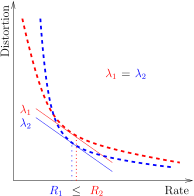
\includegraphics[width=1.0\textwidth]{graphics/RD_slopes} 
  \caption{Two RD (Rate/Distortion) curves.}
  \label{fig:RD_slopes}
\end{figure}

RDO is a process that arises when we need to encode at the same time
two or more different sources of data, $A$ and $B$. When this happens,
each source has own charateristic RD curve (see the
Fig.~\cite{RD_slopes}).

If we suppose now that the contribution to the distortion of the
quantization of each source is independent\footnote{The distortion
generated in one of the sources does not influence the distortion
generated in the other source.} and additive\footnote{Or in general, a
linear combination of the distortions, where each source contributes
more than the other(s) to the total distortion $D$ (this occurs, for
example, when the inverse filters of a linear (orthogonal, backward)
transform has different gains, in which case the quantization step
sizes for a subband should be inversely proportional to the subband
gain).}, that is
\begin{equation}
  D = D^A + D^B,
  \label{eq:additive}
\end{equation}
where $D$ denotes distortion, then the optimal quantization steps must
satisfy that~\cite{vetterli1995wavelets,sayood2017introduction}
\begin{equation}
  \lambda^A_i = \lambda^B_i.
  \label{eq:optimal_quantization}
\end{equation}

To see this, lets suppose that we have used, for example, a set of
quantization step sizes so that $\lambda^A_i/2 = \lambda^B_i,$ and
that we still have room for more bits to encode the frame. In this
situation, the maximum benefit would be obtained if and only if we
decrease $\Delta^A_i$ (modifiying the corresponding
$\mathbf{\Delta}_i$), because the slope for the source $A$ doubles
the slope of the source $B$. Therefore, the optimal quantization
steps are obtained when Eq.~\ref{eq:optimal_quantization} is
true.

\section{Resources}
%{{{ 
\renewcommand{\addcontentsline}[3]{}% Remove functionality of \addcontentsline
\bibliography{data-compression,signal-processing,DWT}
%}}}
